%%%%%%%%%%%%%%%%%%%%%%%%%%%%%%%%%%%%%%%%%
% Full Length Professional CV
% LaTeX Template
% Version 2.0 (13/6/20)
%
% Original author:
% Sreedhar Unnikrishnakurup 
%
% Important note:
% This template requires the my_cv.cls file to be in the same directory as the .tex file. The my_cv.cls file provides the resume style used for structuring the document. THe publication.bib file is needed for adding the publication list
%
%%%%%%%%%%%%%%%%%%%%%%%%%%%%%%%%%%%%%%%%%

%----------------------------------------------------------------------------------------
%	PACKAGES AND OTHER DOCUMENT CONFIGURATIONS
%----------------------------------------------------------------------------------------

\documentclass{my_cv}% Use the custom my_cv.cls style
\begin{document}
\title{CV}
\author{Sreedhar Unnikrishnakurup}
\dob{29 Aug 1984}
\begin{minipage}{0.8\textwidth}
\begingroup
\let\center\flushleft
\let\endcenter\endflushleft
\maketitle
\endgroup
\end{minipage}
\begin{minipage}{0.1\textwidth}
\begin{tikzpicture}[remember picture,overlay]
\clip ($(current page text area.north east)!0.01!(current page text area.south east)!-7.4!(current page text area.north west)$)
  circle (2.1cm) node {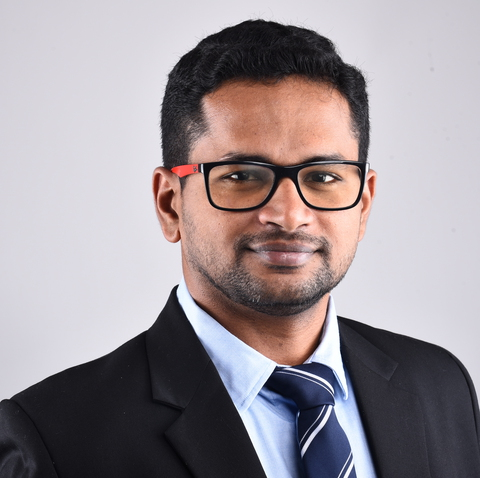
\includegraphics[width=2.3\linewidth]{mypic2}};
\end{tikzpicture}
%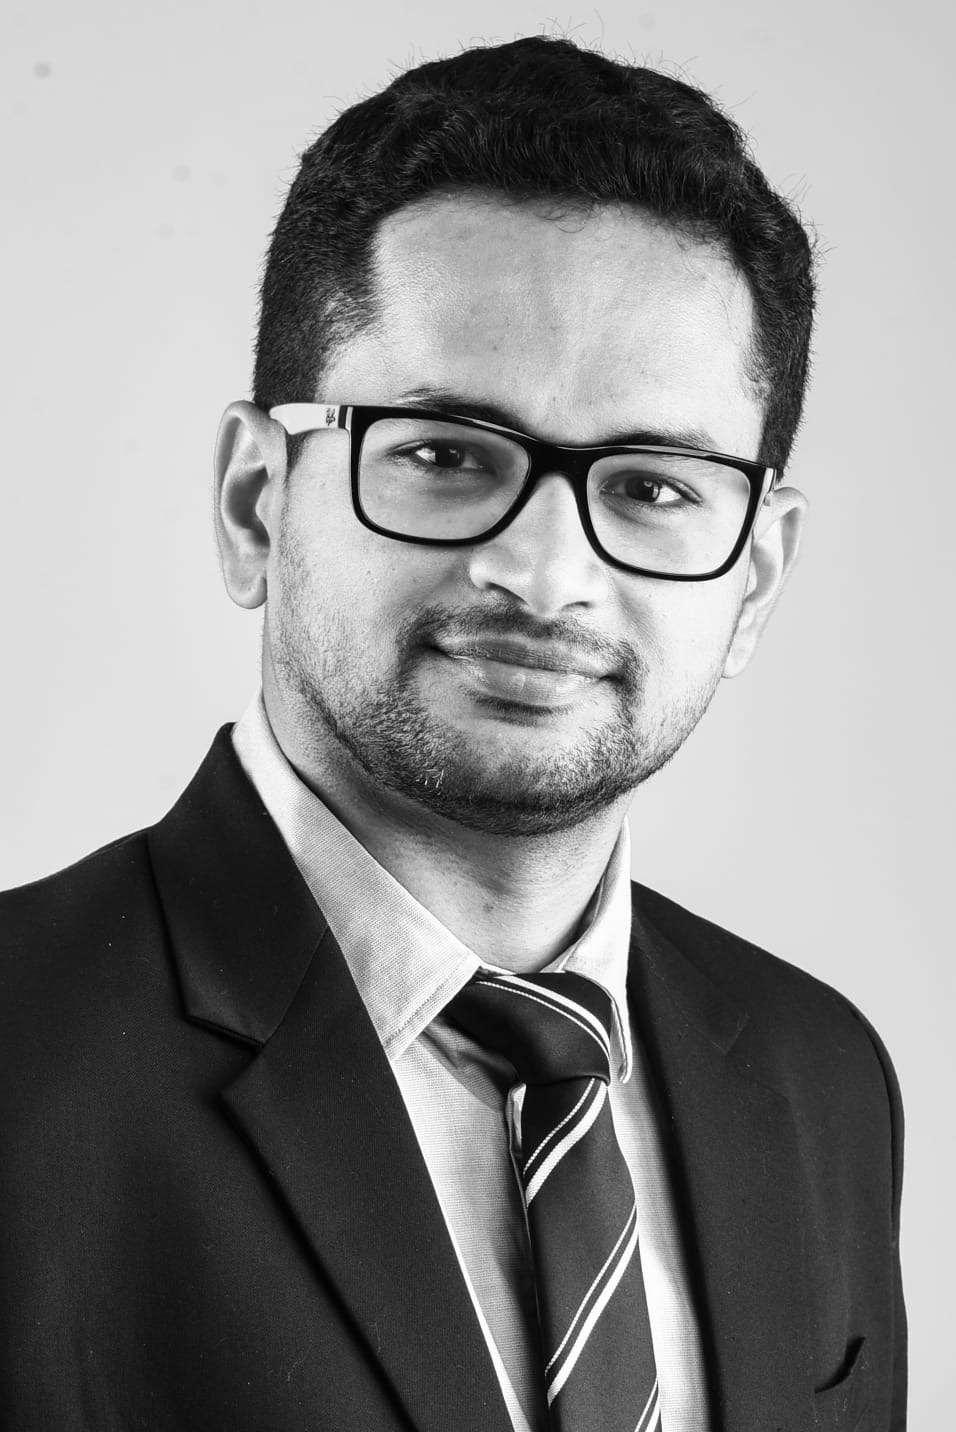
\includegraphics[width=8em]{mypic}
\end{minipage}
\vspace{1.0em}
%-------------------------------------------------------------
%	RESEARCH PROFILE
%-------------------------------------------------------------
\section{Research Profile}
\vspace{0.6em}
\begin{itemize}[leftmargin=0.15in]
\setlength\itemsep{-0.1em}
%\color{mygray}
\item Successfully led and secured \textbf{competitive research funding} as PI and Co-PI, including a multinational grant on curved composite inspection and a collaborative aerospace composite repair project under national R\&D programs.
\item Published \textbf{20 journals and 40 conference papers} in leading outlets focused on thermographic inspection of composites, demonstrating impact in the field of NDT of structural materials; additionally, filed \textbf{12 technology disclosures}, with one licensed to industry partners for practical implementation.
\item Over \textbf{12 years} of post-PhD experience in advanced NDT, with expertise in Infrared Thermography (Pulsed, Lock-in, Induction, Vibro-, and Laser-based IRT), as well as hands-on work with Hyperspectral imaging, X-ray radiography, and THz imaging.
\item Extensive experimental experience with sensor technologies, especially high-speed infrared cameras, and advanced NDT instrumentation for in-situ and lab-based inspection. \textbf{Level 2 certification} in Infrared Thermography.
\item Proven ability to collaborate with multidisciplinary teams across academia and industry, with research experience spanning Europe and Asia.
\end{itemize}

%-------------------------------------------------------------
%	RESEARCH SPECIALIZATIONS & KEYWORDS
%-------------------------------------------------------------
\section{Research Specializations}
\vspace{0.6em}
\begin{itemize}[leftmargin=0.15in]
\setlength\itemsep{-0.1em}
\color{mygray}
\item \textbf{Non-Destructive Testing \& Evaluation (NDT\&E):} Active Infrared Thermography (Pulsed, Lock-in, Induction, Vibro-, and Laser-Assisted IRT), Hyperspectral \& Multispectral Imaging, Terahertz Time-Domain Spectroscopy (THz-TDS), Shearography, X-ray Radiography \& Computed Tomography (CT).
\item \textbf{Structural Health Monitoring (SHM) \& Advanced Materials:} Polymer Matrix Composites (CFRP/GFRP), Aerospace Composite Repair \& Honeycomb Structures, Lightning Strike \& Impact Damage Assessment, Thermal Barrier Coatings, In-situ Monitoring of Laser Powder Bed Fusion (LPBF) Additive Manufacturing.
\item \textbf{Computational Modeling, Signal Processing \& AI:} Multiphysics Finite Element Modeling (COMSOL), Inverse Heat Conduction \& Anisotropic Heat Diffusion, Thermal Signal Processing, Machine Learning \& Deep Learning for Automated Defect Recognition (ADR).
\end{itemize}

%-------------------------------------------------------------
%	WORK EXPERIENCE SECTION
%-------------------------------------------------------------
\section{Work Experience}
\vspace{0.6em}
\subsection{Senior Scientist}
\subsubsection{\href{https://www.a-star.edu.sg/imre}{Structural Materials Department, Institute of Materials Research and Engineering (IMRE), A*STAR}}
\subsubsection{\href{https://www.a-star.edu.sg/imre/feat}{Future Energy Acceleration and Translation (FEAT) Centre, IMRE, A*STAR} {\normalfont\color{mygray}(2026--Ongoing)}}
\datedsubsection{Apr 2024--Ongoing}{Singapore}
%\paragraph{
\definecolor{mypink}{rgb}{0.86, 0.08, 0.24} % Define a pink color
\hypersetup{
    colorlinks=true, % Enables colored links
    linkcolor=mypink, % Makes references (hyperref) pink
    urlcolor=blue,   % Keeps URLs in blue
    citecolor=black  % Keeps citations black
}
\begin{itemize}[leftmargin=0.15in]
\setlength\itemsep{-0.1em}
\color{mygray}
\item \href{https://www.a-star.edu.sg/imre/feat}{Future Energy Acceleration and Translation (FEAT) Centre} (\textbf{AMOFES} \& \textbf{STRIDE} Projects): Advanced non-destructive evaluation and pulsed laser thermography characterization of extreme-environment and fusion energy materials, including interfacial thermal resistance assessment of tungsten coatings on boron carbide substrates [\textcolor{mypink}{\hyperref[C2]{C2}}].
\item \href{https://www.a-star.edu.sg/aerospace}{Singapore Aerospace Programme (SAP)} (Co-PI): UD-CFRP cross-ply laminate characterization using Induction Thermography for aerospace composite repair [\textcolor{mypink}{\hyperref[J3]{J3}}, \textcolor{mypink}{\hyperref[J6]{J6}}, \textcolor{mypink}{\hyperref[C6]{C6}}].
\item Material Informed Differential Generative AI (\href{https://aisingapore.org/design-beyond-what-you-know-material-informed-differential-generative-ai-midgai-for-light-weight-high-entropy-alloys-and-multi-functional-composites/}{MIDGAI}) for Multi-functional Composites (Project Member): Development of high-strength and high-conductivity composites using generative AI.
\item Lead Researcher on Advanced NDT Projects: Multimodal NDE using IRT, Ultrasonic, and Shearography of lightning strike damage in painted CFRP laminates with lightning strike protection [\textcolor{mypink}{\hyperref[J1]{J1}}]; sweep-excited vibrothermography and machine learning for low-energy impact damage in carbon composites [\textcolor{mypink}{\hyperref[C3]{C3}}]; infrared thermography diagnostics for reverse-bias stability in perovskite solar modules [\textcolor{mypink}{\hyperref[J2]{J2}}]; water ingress detection in honeycomb sandwich aircraft structures; evaluation of cold-sprayed coating porosity [\textcolor{mypink}{\hyperref[J5]{J5}}]; sub-coating crack detection in metallic components using induction IRT; and physics-informed AI/deep learning for automated defect detection in IRT [\textcolor{mypink}{\hyperref[J4]{J4}}].
\end{itemize}%}
{\color{mygray1} \hdashrule[0.1ex]{18.8cm}{0.2mm}{1mm}}
%-----------------------------------------------------------------------
\subsection{Scientist}
\subsubsection{\href{https://www.a-star.edu.sg/imre}{Structural Materials Department, Institute of Materials Research and Engineering (IMRE), A*STAR}}
\datedsubsection{Nov 2021--Mar 2024}{Singapore}
\begin{itemize}[leftmargin=0.15in]
\setlength\itemsep{-0.1em}
\color{mygray}
\item Project \href{https://www.a-star.edu.sg/imre/news-and-highlights/highlights/media/polymer-matrix-composites-programme-(pmcp)}{Polymer Matrix Composites Programme (PMCP)} (Work Package Lead): Managed work package involving in-line IRT monitoring of prepreg manufacturing, characterization of impact and manufacturing damages in CFRP [\textcolor{mypink}{\hyperref[J7]{J7}}, \textcolor{mypink}{\hyperref[C4]{C4}}, \textcolor{mypink}{\hyperref[C12]{C12}}], inspection of filament-wound GFRP pipes, and impact damage characterization using Induction IRT.
\item Principal Investigator (PI) on Multinational Collaborative Grant: Developed quantitative active thermography and optical profile correction methods for inspecting complex curved aerospace composite structures [\textcolor{mypink}{\hyperref[C5]{C5}}, \textcolor{mypink}{\hyperref[C7]{C7}}, \textcolor{mypink}{\hyperref[C8]{C8}}].
\end{itemize}
{\color{mygray1} \hdashrule[0.1ex]{18.8cm}{0.2mm}{1mm}}
%-----------------------------------------------------------------------
\subsection{Visiting Researcher}
\subsubsection{\href{https://www.dmmm.poliba.it/index.php/en/}{Mechanical Design and Machine Construction (IIND-03/A) NDT Research Group, Politecnico di Bari}}
\datedsubsection{November 2025 - February 2026}{Bari, Italy}
\begin{itemize}[leftmargin=0.15in]
\setlength\itemsep{-0.1em}
\color{mygray}
\item Thermal Signature Analysis for Defect Detection in Laser-Based Additive Manufacturing [\textcolor{mypink}{\hyperref[C1]{C1}}]
\item Development of Machine Learning Algorithms for the inline monitoring of LPBF process
\end{itemize}
{\color{mygray1} \hdashrule[0.1ex]{18.8cm}{0.2mm}{1mm}}
%------------------------------------------------------------
\subsection{Senior Project Officer}
\subsubsection{\href{https://www.cnde.in/}{Centre for Non-Destructive Evaluation (CNDE), IIT Madras}}
\datedsubsection{May 2018 - Sep 2021}{Chennai, India}
%\paragraph{
\begin{itemize}[leftmargin=0.15in]
\setlength\itemsep{-0.1em}
\color{mygray}
\item Application of Nondestructive IRT testing for thickness inspection of thermal barrier coatings and validation using THz-TDS and Eddy current testing [\textcolor{mypink}{\hyperref[J12]{J12}}].
\item Composite inspection using induction heating IRT. [\textcolor{mypink}{\hyperref[J9]{J9}}]
\item Crack inspection in steel billets at elevated temperatures using Laser assisted IRT [\textcolor{mypink}{\hyperref[J14]{J14}}].
\item Development of artificial intelligence-assisted advanced X-ray radiography imaging and automatic defect recognition of critical welds and high-energy materials [\textcolor{mypink}{\hyperref[J10]{J10}}]
\item Numerical investigation of anisotropic heat diffusion in polycrystalline and composite microstructures [\textcolor{mypink}{\hyperref[J13]{J13}}].
\end{itemize}%}
{\color{mygray1} \hdashrule[0.1ex]{18.8cm}{0.2mm}{1mm}}
%{\color{mygray} \rule{\linewidth}{0.5mm} }
%-----------------------------------------------------------------
\subsection{Cohort Member BA3}
\subsubsection{\href{https://www.joinef.com/}{Entrepreneur First}}
\datedsubsection{February 2020 - May 2020}{Bangalore, India}
\begin{itemize}[leftmargin=0.15in]
\setlength\itemsep{-0.1em}
\color{mygray}
\item Explored several interesting technological solutions, exploring the market, validating the technology, speaking to customers, and researching prototypes
\item The ideas that we worked on is, detect and report quality-compromised and counterfeit drugs using a mobile cloud-based cost-effective hyper-spectral Imaging based AI device
\end{itemize}
{\color{mygray1} \hdashrule[0.1ex]{18.8cm}{0.2mm}{1mm}}
%------------------------------------------------------------------
\subsection{Postdoctoral Research Scientist}
\subsubsection{\href{https://www.bam.de/Navigation/DE/Home/home.html}{NDT group 8.7, Federal Institute for Material Research and Testing (BAM)}}
\datedsubsection{January 2016 - June 2017}{Berlin, Germany}
\begin{itemize}[leftmargin=0.15in]
\setlength\itemsep{-0.1em}
\color{mygray}
\item Project \href{http://projects.npl.co.uk/vitcea/}{VITCEA} (Validated Inspection Techniques for Composites in Energy Applications) 
\item Optimize and validate active thermography as full-field, fast and non-contact NDE technique for quantitative testing of FRP structures [\textcolor{mypink}{\hyperref[J16]{J16}}]
\item Laser Thermography for surface crack detection at high temperature [\textcolor{mypink}{\hyperref[C23]{C23}}]
\end{itemize}
{\color{mygray1} \hdashrule[0.1ex]{18.8cm}{0.2mm}{1mm}}
%-----------------------------------------------------------------------
\subsection{Visiting Research Scientist}
\subsubsection{\href{https://innowacje.zut.edu.pl/cooperationoffer/electromagnetic-methods-non-destructive-testing}{Electromagnetic NDT Research Group, West Pomeranian University (ZUT)}}
\datedsubsection{January 2015 - March 2015}{Szczecin, Poland}
\begin{itemize}[leftmargin=0.15in]
\setlength\itemsep{-0.1em}
\color{mygray}
\item Scientific Exchange as part of \href{https://cordis.europa.eu/project/id/269202/results}{FP7 Project: Health Monitoring of Offshore Wind Farms (HEMOW)}
\item Terahertz imaging and time domain analysis for material defect identification in Composite Wind turbine blades [\textcolor{mypink}{\hyperref[C33]{C33}}]
\item Active Infrared Thermography for defect identification in composite materials - Numerical investigations of heat sink effects in the infrared inspecton of composites [\textcolor{mypink}{\hyperref[C29]{C29}}, \textcolor{mypink}{\hyperref[C34]{C34}}]
\end{itemize}
{\color{mygray1} \hdashrule[0.1ex]{18.8cm}{0.2mm}{1mm}}
%------------------------------------------------------------------------
\subsection{Institute Postdoctoral Fellow}
\subsubsection{\href{https://www.cnde.in/}{Centre for Non-Destructive Evaluation (CNDE), IIT Madras}}
\datedsubsection{September 2014 - December 2015}{Chennai, India}
\begin{itemize}[leftmargin=0.15in]
\setlength\itemsep{-0.1em}
\color{mygray}
\item Numerical modelling of microstructural heat diffusion and ultrasonic wave propagation in Polycrystalline Materials [\textcolor{mypink}{\hyperref[C25]{C25}}, \textcolor{mypink}{\hyperref[C27]{C27}}, \textcolor{mypink}{\hyperref[C28]{C28}}]
\item CMT welding process monitoring using IR thermography [\textcolor{mypink}{\hyperref[J18]{J18}}, \textcolor{mypink}{\hyperref[C21]{C21}}, \textcolor{mypink}{\hyperref[C24]{C24}}]
\item In-line laser thermography for Online Monitoring of steel billets to predict the surface cracks formed during the non-uniform cooling [\textcolor{mypink}{\hyperref[C26]{C26}}, \textcolor{mypink}{\hyperref[C30]{C30}}]
\end{itemize}
{\color{mygray1} \hdashrule[0.1ex]{18.8cm}{0.2mm}{1mm}}
%------------------------------------------------------------------------
\subsection{Research Associate}
\subsubsection{\href{https://www.cnde.in/}{Centre for Non-Destructive Evaluation (CNDE), IIT Madras}}
\datedsubsection{April 2007 - December 2008}{Chennai, India}
\begin{itemize}[leftmargin=0.15in]
\setlength\itemsep{-0.1em}
\color{mygray}
\item Development of online weld quality monitoring for AA2219 liquid propellant tanks using Infrared Thermal Imaging and X-ray radiography [\textcolor{mypink}{\hyperref[J20]{J20}}]
\item Developed a finite element model for the prediction of temperature profiles during welding
\end{itemize}
%-------------------------------------------------------------
%	EDUCATION SECTION
%-------------------------------------------------------------
\section{Education}
\vspace{1em}
\subsection{\href{https://adum.fr/as/ed/cv.pl?mat=39446&site=adumR} {Ph.D. in Mechanics \& Civil Engineering}}
\subsubsection{\faInstitution \hspace{0.2em} \href{https://www.umontpellier.fr/en/}{Department of Mechanics and Civil Engineering (LMGC), University of Montpellier 2 (UM2), France}}
\datedsubsection{2011 - 2014}{Montpellier, France}
\begin{itemize}[leftmargin=0.15in]
\setlength\itemsep{-0.1em}
\color{mygray}
\item Dissertation Topic: \href{https://bit.ly/2UFQyFi}{Weld pool shape identification using Multi-physics modelling and Experiments} [\textcolor{mypink}{\hyperref[J17]{J17}}, \textcolor{mypink}{\hyperref[C35]{C35}}-\textcolor{mypink}{\hyperref[C39]{C39}}]
\end{itemize}
{\color{mygray1} \hdashrule[0.1ex]{18.8cm}{0.2mm}{1mm}}
%-------------------------------------------------------------------------------
\subsection{M.S. in Mechanical Engineering}
\subsubsection{\faInstitution \hspace{0.2em} \href{https://www.iitm.ac.in/}{Department of Mechanical Engineering, Indian Institute of Technology Madras (IIT Madras), India}}
\datedsubsection{2008 - 2010}{Chennai, India}
\begin{itemize}[leftmargin=0.15in]
\setlength\itemsep{-0.1em}
\color{mygray}
\item Dissertation Topic: Online weld quality monitoring using Infrared Thermal Imaging [\textcolor{mypink}{\hyperref[J19]{J19}}, \textcolor{mypink}{\hyperref[J20]{J20}}, \textcolor{mypink}{\hyperref[C32]{C32}}, \textcolor{mypink}{\hyperref[C40]{C40}}]
\end{itemize}
{\color{mygray1} \hdashrule[0.1ex]{18.8cm}{0.2mm}{1mm}}
%--------------------------------------------------------------------------------
\subsection{Bachelors in Mechanical Engineering}
\subsubsection{\faInstitution \hspace{0.2em} \href{https://www.ieindia.org/webui/iei-home.aspx}{Department of Mechanical Engineering, Institution of Engineers (India), India}}
\datedsubsection{2002 - 2006}{Kottayam, India}
\newpage
%--------------------------------------------------------------
%	                 Honors, Awards and Competitive Grants
%-------------------------------------------------------------
\section{Honors, Awards and Competitive Grants}
\vspace{0.6em}
\grantsubsection{Conference Co-Chair, Asian Quantitative Infrared Thermography Conference (QIRT-Asia 2027), Singapore}{2027}
\grantsubsection{Invited Speaker Recognition, NDE 2026 Conference, Indian Society for Non-Destructive Testing (ISNT)}{2026}
\grantsubsection{Visiting Researcher Fellowship, NDT Research Group, Politecnico di Bari, Italy}{2025--2026}
\grantsubsection{Technology Commercialization \& Licensing Recognition (1 TD Licensed, 12 TDs Filed), IMRE, A*STAR}{2021--2026}
\grantsubsection{Steering Committee Member, Quantitative InfraRed Thermography (QIRT \& QIRT-Asia)}{2023--Present}
\grantsubsection{Co-Principal Investigator, Singapore Aerospace Programme (SAP) Research Grant, A*STAR}{2022--2026}
\grantsubsection{Principal Investigator, Multinational Grant on Curved Aerospace Composite Inspection, A*STAR}{2022--2025}
\grantsubsection{Work Package Lead, Polymer Matrix Composites Programme (PMCP), A*STAR, Singapore}{2021--2025}
\vspace{0.2em}
%-------------------------------------------------------------
%	             INVITED PRESENTATIONS
%-------------------------------------------------------------
\section{Invited Presentations}
\vspace{0.3em}
\begin{itemize}[leftmargin=0.15in]
\setlength\itemsep{-0.15em}
\color{mygray}
\item \textbf{Invited Speaker}, NDE 2026 Conference \& Exhibition, Organized by Indian Society for Non-Destructive Testing (ISNT), Hyderabad, India, November 14--17, 2026.
\item \textbf{Invited Research Seminar}, Mechanical Design and Machine Construction (IIND-03/A) NDT Research Group, Department of Mechanics, Mathematics and Management (DMMM), Politecnico di Bari, Talk: \textit{Thermal Signature Analysis and Machine Learning for In-line Monitoring of Additive Manufacturing}, Bari, Italy, 2025--2026.
\item \textbf{Invited Tutorial Speaker}, Preconference Tutorials, NDE 2019 Organized by Indian Society for Non-Destructive Testing (ISNT), Talk: \textit{Applications of Thermal Imaging in Aerospace Industry}, Bengaluru, India, December 3, 2019.
\item \textbf{Invited Speaker}, Workshop on Advanced NDE Techniques and Applications organized by TATA STEEL, Talk: \textit{Advanced Thermography Techniques}, TATA Nagar, Jamshedpur, India, August 17, 2015.
\item \textbf{Invited Speaker}, Polish Society for Theoretical and Applied Electrical Engineering Section in Szczecin (PTETiS), Talk: \textit{Research and Development in the Field of NDE @ CNDE}, West Pomeranian University of Technology, Szczecin, Poland, March 12, 2015.
\item \textbf{Invited Speaker}, Polish Society for Nondestructive Testing and Technical Diagnostics Section in Szczecin (PTBNiDT), Talk: \textit{Research and Applications of IR Thermography @ CNDE}, Szczecin, Poland, February 26, 2015.
\end{itemize}
%-------------------------------------------------------------
%	                 Certifications and Courses
%-------------------------------------------------------------
\section{Certifications and Memberships}
\vspace{0.3em}
\begin{itemize}[leftmargin=0.15in]
\setlength\itemsep{-0.15em}
\color{mygray}
\item[\faCertificate] Infrared Thermography Level 2 Certification. Issued on October 2026
\item[\faCertificate] Project Management Fundamentals by EPM. Issued on October 2022
\item[\faCertificate] Infrared Thermography Level 1 by Infrared Training Center. Issued on May 2022
\item[\faCertificate] Deep Learning, a 5-course specialization by deeplearning.ai on Coursera. Specialization Certificate earned on September 23, 2018
\item [\faUsers] Technical Committee Member, ISO/TC 135/SC 8 -- Thermographic Testing
\item [\faUsers] Member of ASTM International
\item [\faUsers] Quantitative InfraRed Thermography (QIRT) Steering Committee Member
\item [\faUsers] Asian Quantitative Infrared Thermography (QIRT-Asia) Steering Committee Member
\item [\faUsers] Member of Non-Destructive Testing Society Singapore (NDTSS)
\item [\faUsers] Member of Indian Society for Non-Destructive Testing (ISNT)
\item [\faUsers] Member of Institution of Engineers (India), and Chartered Engineer Certification
\end{itemize}
%----------------------------------------------------------------
%	Mentoring Activities
%----------------------------------------------------------------
\section{Mentoring}
\vspace{0.3em}
\noindent \faEye \hspace{1em} \color{mygray} During postdoctoral tenure at IIT Madras: 4 Ph.D. Students and 2 Master student 
\begin{itemize}[leftmargin=0.15in]
\setlength\itemsep{-0.15em}
\color{mygray}
\item Shivaprasad S (Ph.D.) - Voronoi Cell based FEM simulations for wave propagation in solids [\textcolor{mypink}{\hyperref[C25]{C25}}, \textcolor{mypink}{\hyperref[C27]{C27}}]
\item Renil Thomas K (Ph.D.) - Induction thermography inspection of CFRP and CMT weld monitoring [\textcolor{mypink}{\hyperref[J3]{J3}}, \textcolor{mypink}{\hyperref[J6]{J6}}, \textcolor{mypink}{\hyperref[J9]{J9}}, \textcolor{mypink}{\hyperref[J18]{J18}}] 
\item Nithin P V (Ph.D.) - Laser thermography for crack inspection in steel samples at elevated temperature [\textcolor{mypink}{\hyperref[J14]{J14}}, \textcolor{mypink}{\hyperref[J15]{J15}}]
\item Surendra Gupta (Ph.D.) - Emissivity characterization of nano photonic emitters [\textcolor{mypink}{\hyperref[J11]{J11}}]
\item Anurag Saini (MTech) - Numerical investigation of Heat diffusion in particle reinforced composite [\textcolor{mypink}{\hyperref[J13]{J13}}]
\item Dhruv Gamdha (MTech) - Ray tracing model for X-ray simulation and AI based automatic defect Recognition [\textcolor{mypink}{\hyperref[J10]{J10}}]
\end{itemize}
%-------------------------------------------------------------
%	Publication
%-------------------------------------------------------------
\section{Publication}
\vspace{0.5em}
\nobibliography{publication}
\bibliographystyle{unsrtnat}
\subsection{\faFileTextO \hspace{0.5em}\bfseries Journal Articles}
\vspace{0.3em}
\renewcommand{\theenumi}{J\arabic{enumi}} % Change numbering format to J1, J2, ...
\begin{enumerate}
\setlength\itemsep{-0.18em}
\color{mygray}
 \item \label{J1} \bibentry{unnikrishnakurup2026multimodal}
 \item \label{J2} \bibentry{Wang2026NatureEnergy}
 \item \label{J3} \bibentry{unnikrishnakurup2025assessment} 
 \item \label{J4} \bibentry{bounenni2024advanced} 
 \item \label{J5} \bibentry{unnikrishnakurup2024exploring} 
 \item \label{J6} \bibentry{kidangan2024uncovering} 
 \item \label{J7} \bibentry{kidangan2024induction} 
 \item \label{J8} \bibentry{Mercy2022} 
 \item \label{J9} \bibentry{Renil2022} 
 \item \label{J10} \bibentry{Dhruv2021} 
 \item \label{J11} \bibentry{Surendra2021} 
 \item \label{J12} \bibentry{Sreedhar2020} 
 \item \label{J13} \bibentry{Saini2020} 
 \item \label{J14} \bibentry{puthiyaveettil2020} 
 \item \label{J15} \bibentry{Nithin2019} 
 \item \label{J16} \bibentry{maierhofer2018} 
 \item \label{J17} \bibentry{unnikrishnakurup2017} 
 \item \label{J18} \bibentry{thomas2017} 
 \item \label{J19} \bibentry{sreedhar2016} 
 \item \label{J20} \bibentry{sreedhar2012} 
\end{enumerate}

\subsection{\faFilePowerpointO \hspace{0.5em}\bfseries Conference Presentations}
\renewcommand{\theenumi}{C\arabic{enumi}} % Change numbering format to C1, C2, ...
\begin{enumerate}
\setlength\itemsep{-0.18em}
\color{mygray}
\item \label{C1} \bibentry{daccardi2026multilayer}
\item \label{C2} \bibentry{unnikrishnakurup2026pulsed}
\item \label{C3} \bibentry{unnikrishnakurup2026enhancing}
\item \label{C4} \bibentry{unnikrishnakurup2025lockin}
\item \label{C5} \bibentry{zheng2024multispectral}
\item \label{C6} \bibentry{unnikrishnakurup2023characterizing}
\item \label{C7} \bibentry{gnessougoucurved}
\item \label{C8} \bibentry{unnikrishnakurup1exploring}
\item \label{C9} \bibentry{kumara2022dynamic}
\item \label{C10} \bibentry{zheng2022using}
\item \label{C11} \bibentry{unnikrishnakurup2022crack} 
\item \label{C12} \bibentry{Sreeconf2022} 
\item \label{C13} \bibentry{Jyoticonf2020} 
\item \label{C14} \bibentry{Surendraconf2020} 
\item \label{C15} \bibentry{Dhruv2019} 
\item \label{C16} \bibentry{Sreedharconf2020} 
\item \label{C17} \bibentry{Sruthiconf2018} 
\item \label{C18} \bibentry{Nithinconf2018} 
\item \label{C19} \bibentry{Maierhoferconf2018} 
\item \label{C20} \bibentry{Krishnaconf2017} 
\item \label{C21} \bibentry{Renilconf2016} 
\item \label{C22} \bibentry{Nithinconf2016} 
\item \label{C23} \bibentry{Polomskiconf2016} 
\item \label{C24} \bibentry{Kidanganconf2016} 
\item \label{C25} \bibentry{Shivaprasadconf2015} 
\item \label{C26} \bibentry{Sreedharconf2015} 
\item \label{C27} \bibentry{Shivaprasadcomsolconf2015} 
\item \label{C28} \bibentry{SreedharQIRTconf2015} 
\item \label{C29} \bibentry{SzymznikQIRTconf2015} 
\item \label{C30} \bibentry{SreeQIRTconf2015} 
\item \label{C31} \bibentry{SreeSGRconf2015} 
\item \label{C32} \bibentry{SreePolandconf2015} 
\item \label{C33} \bibentry{Chadyconf2015} 
\item \label{C34} \bibentry{Barbaraconf2014} 
\item \label{C35} \bibentry{Rouquetteconf2014} 
\item \label{C36} \bibentry{Sreedharconf2013} 
\item \label{C37} \bibentry{Sreedharconf2012} 
\item \label{C38} \bibentry{SreedharNconf2012} 
\item \label{C39} \bibentry{Rouquetteconf2011} 
\item \label{C40} \bibentry{Sreedharconf2009} 
\end{enumerate}

\subsection{\faLightbulbO \hspace{0.5em}\bfseries Innovation and Technology Transfer}

\begin{itemize}
\setlength\itemsep{-0.1em}
  \item Filed \textbf{12 Technology Disclosures} at Institute of Materials Research and Engineering (IMRE), A*STAR between 2021--2026 in the areas of Infrared Thermography, Composite Inspection, and Laser-Based NDT.
  \item \textbf{1 TD licensed} to industry partner for use in  composite inspection workflows in bicycle repair.
\end{itemize}
%-------------------------------------------------------------
\end{document}
